\documentclass[12pt]{article}
\usepackage{fancyhdr}
\usepackage{color}
\usepackage{multicol}
\usepackage{enumitem}
\usepackage{graphicx}
\usepackage{sectsty}
\usepackage{array}
\usepackage{tikz}

\allsectionsfont{\centering}

\usepackage{draftwatermark}
	\SetWatermarkText{\copyright wolf-math.com}
	\SetWatermarkScale{4}
	\SetWatermarkLightness{1}

\usepackage[margin=1in, headsep=0pt]{geometry}
\setlength{\parindent}{0cm}
\pagestyle{empty}


\begin{document}

Mr. Wolf \\ Algebra 2 \\ CMSD-JFK\\2014-2015



\section*{Rational Exponents \& Radicals}



	\textbf{SWBAT} simplify exponential expressions by properly using properties of exponents.\\
	
	\textbf{SWBAT} simplify radical expressions by factoring out perfect roots of the radical.\\
	
	\textbf{SWBAT} simplify radical expressions using properties of radicals.\\
	
	\textbf{SWBAT} convert from radical form to rational exponent form.\\
	
	\textbf{SWBAT} simplify rational exponents using properties of exponents\\
	
	\textbf{SWBAT} evaluate rational exponential expressions by breaking them apart into the product property.
	


\subsection*{Standards}
	\textbf{Real Number System \hfill N-RN.1}\\
	
	 Explain how the definition of the meaning of rational exponents follows from extending the properties of integer exponents to those values, allowing for a notation for radicals in terms of rational exponents. For example, we define $5^{\frac{1}{3}}$ to be the cube root of 5 because we want $\left(5^{\frac{1}{3}}\right)^{3} =\left(5^{\frac{1}{3}}\right)^{3}$ to hold, so $\left(5^{\frac{1}{3}}\right)^{3}$ must equal 5. \\
	
2.	 Rewrite expressions involving radicals and rational exponents using the properties of exponents.
	



\subsection*{Pre-Assessment} To introduce our topic of exponential functions the students will begin by learning properties of exponents. The students should have already encountered this before, but since this information is necessary for our topic we will review the content and make sure that there are absolutely no misconceptions.  
	


\subsection*{Assessments} Homework will be graded, there will be a lab, and test on this material. 
	


\subsection*{Before \& After}

	\textbf{Before} the students learned about creating algebraic expressions that represent a rule. This lesson prepares students for the extention of those that we just learned in our first unit. While we were learning about arithmetic functions before, we are now moving towards exponential functions.\\
	


	\textbf{After} we will be learning how to solve for an exponential expression. This requires knowledge of the properties of exponents and rational exponents. From there we will analyze and model exponential functions.
	

	
\subsection*{Differentiation} After students learn the certain properties they will go on to do group work in stations. In these stations they will work on enriching their understanding of the aim by working collaboratively to solve a harder list of problems. Within each station the problems get harder requiring very little effort for the first question and a lot of effort for the last question.\\

\let\stdsection\section
\renewcommand\section{\newpage\stdsection}

\section*{Properties of Exponents}


\begin{enumerate}
\setlength\itemsep{1cm}

	\item \textbf{Product Property:} $a^m \cdot a^n= a^{m+n}$\hspace{1cm} \textbf{and} \hspace{1cm} $(xy)^m=x^m \cdot y^m$ \\
	
		\hspace{.6in} Example: $2^6 \cdot 2^8=2^{14}$\hspace{1cm}   \textbf{ and}  \hspace{1cm}  $(2x)^{5}=2^5 \cdot x^5$\\ 
	
	\item \textbf{Power Property:} $\left(a^m \right)^n = a^{(m \cdot n)}$\\
	
		\hspace{.6in} Example: $\left(g^2\right)^3=g^6$\\ 
	
	\item \textbf{Quotient Property:} $\frac{a^m}{a^n}=a^{m-n}$\\
	
		\hspace{.6in} Example: $\frac{k^7}{k^4} = k^3$ and $\frac{k^2}{k^8}=k^{-6}$\\ 
	
	\item \textbf{Negative Property:} $a^{-n}=\frac{1}{a^n}$ and $\frac{1}{a^{-n}}=a^{n}$ \\
	
		\hspace{.6in} Example: $2^{-1}=\frac{1}{2}$\hspace{1cm} \textbf{and} \hspace{1cm} $\left(\frac{1}{2}\right)^{-1}=2$ \hspace{1cm} \textbf{and} \hspace{1cm} $\left(\frac{2}{3}\right)^{-1}=\frac{3}{2}$\\ 
	
	\item \textbf{Zero Property:} $a^0=1$\\
		
		\hspace{.6in} Example: $555,987,123,987,123^0=1$\\ 
	
	\item \textbf{Power of a Quotient Property:} $\left(\frac{a}{b}\right)^n=\frac{a^n}{b^n}$\\
	
		\hspace{.6in} Example: $\left(\frac{2}{3}\right)^3=\frac{2^3}{3^3}=\frac{8}{27}$ \\

\end{enumerate}

\pagebreak



\subsection*{Board Work}

Simplify each expression.\\

\begin{enumerate}

	\item $f^3 \cdot f^5=$\\
	
	\item $7^3 \cdot 7^7=$\\
	
	\item $(bc)^5=$\\
	
	\item $(2g)^3=$\\
	
	\item $u^{9^{10}}=$\\
	
	\item $ 4^{2^5}=$\\
	
	\item $\frac{v^8}{v^2}=$\\
	
	\item $\frac{v^2}{v^8}=$\\
	
	\item $\left(\frac{2}{3}\right)^4=$\\
	
	\item $q^{-1}=$\\
	
	\item $6^{-3}=$\\
	
	\vspace{1cm}
	
	Challenge problem: $\frac{9x^2y^3z^{2}}{3xy^{-5}z^{6}}=$\\

\end{enumerate}	
	
\pagebreak

\subsection*{You Try: Station Work}


\textbf{Station 1: Multiplication--} Simplify each product of exponents. Leave answers in exponential form.\\

Example 1: $x^5 \cdot x^2=x^7$\\

\begin{enumerate}
\begin{multicols}{2}

	\item $ y^6 \cdot y^4 =\underline{\hspace{1in}}$\\
	
	\item $(7h)^3=\underline{\hspace{1in}}$\\
	
	\item $ 5^{3} \cdot (5n)^2=\underline{\hspace{1in}}$\\
	
	\item $ (2n)^{3} \cdot 2^2 = \underline{\hspace{1in}}$\\

\end{multicols}
\end{enumerate}


\hrulefill

\textbf{Station 2: Fractions \& division -- } Simplify each expression. Make sure there are no negative exponents. Leave answers in exponential form.\\ 

\begin{enumerate}[resume]
\begin{multicols}{2}

	\item $\left(\frac{1}{n}\right)^{3}=\underline{\hspace{1in}}$\\
	
	\item $\frac{p^6}{p^3}=\underline{\hspace{1in}}$\\
	
	\item $\frac{h^9}{h^{12}}=\underline{\hspace{1in}}$\\
	
	\item $\left(\frac{2^2m^3n^{2}}{2mn^2}\right)=\underline{\hspace{1in}}$\\

\end{multicols}
\end{enumerate}

\hrulefill

\textbf{Station 3: Negative and Zero Exponents --} Simplify each expression so that there are no negative exponents. Leave answers in exponential form.

\begin{enumerate}[resume]
\begin{multicols}{2}

	\item $6^{-2}=\underline{\hspace{1in}}$\\

	\item $(bagillion)^0=\underline{\hspace{1in}}$\\
	
	\item $\left(\frac{1}{10}\right)^{-3}=\underline{\hspace{1in}}$\\
	
	\item $\left(\frac{7}{2}\right)^{2}=\underline{\hspace{1in}}$\\
	
	
\end{multicols}
\end{enumerate}

\hrulefill

\textbf{Station 4: Powers of exponents--} Simplify so that there is only one level of exponent (e.g. \textbf{don't} write $2^{2^2}$ as an answer). Leave answers in exponential form.

\begin{enumerate}[resume]
\begin{multicols}{2}

	\item $\left(2^2\right)^2=\underline{\hspace{1in}}$\\
	
	\item $\left(c^5\right)^7=\underline{\hspace{1in}}$\\
	
	\item $\left(\frac{1}{2}\right)^{10}=\underline{\hspace{1in}}$\\
	
	\item $\left(\left(\frac{3}{4}\right)^{-1}\right)^{-1}=\underline{\hspace{1in}}$\\

\end{multicols}
\end{enumerate}

\pagebreak

\section*{Square Roots}

Square Roots are the opposite of squares (exponent of 2). This is also called an \textit{inverse}.\\

\begin{LARGE}
	$$\sqrt{a^2}=a$$
\end{LARGE}



\hrulefill

There are 2 parts to a squareroot.

\begin{enumerate}

	\item the \textit{RADICAL}\\
	
	\item the \textit{RADICAND}\\
	
\end{enumerate}

\begin{center}
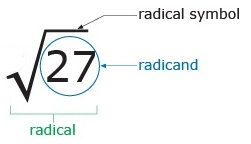
\includegraphics[scale=.7]{squareroot.jpg}
\end{center}


The \textit{radical} tells us that we're looking for identical factors.\\

the \textit{radicand} is a number that needs to be factored so we can pull out the identical ones.\\

\textbf{Example:} $\sqrt{25}=\sqrt{5\cdot5} \Longrightarrow$ since there are 2 5's $\Longrightarrow \sqrt{5\cdot5}=5$\\

\pagebreak

\section*{Simplifying Square Root Expressions}

\begin{center}
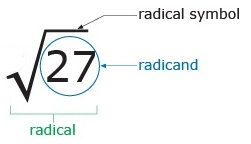
\includegraphics[scale=.7]{squareroot.jpg}\\
\end{center}

To simplify radical expressions follow these steps\\

\textbf{Step 1:} factor the radicand\\

\textbf{Step 2:} pull out factors that a repeated twice.\\

\textbf{Step 3:} all other factors stay inside the radical\\

\hrulefill

\textbf{Examples:} Simplify the square root.\\

\begin{multicols}{2}
\textbf{We try:}\\

\begin{enumerate}
	\setlength\itemsep{1cm}

	\item $\sqrt{36}$\\
	
	
	\item $\sqrt{50}$\\
	
	
	\item $\sqrt{27}$\\
	
	
	\item $\sqrt{27x^2}$\\
	
		
\textbf{You Try:}\\
	
	\item  $\sqrt{120}$ \\
	
	
	\item $\sqrt{52y^4}$\\
	
	
	\item $\sqrt{16}$\\
	
	
	\item $\sqrt{160n^7}$\\
	
	

\end{enumerate}
\end{multicols}

 \textbf{Challenge Problem:} $\sqrt[5]{800h^{11}}$

\section*{Other Roots}

Roots are the opposite of exponents. This is also called an \textit{inverse}.\\

\begin{LARGE}
	$$\sqrt[n]{a^n}=a$$
\end{LARGE}



\hrulefill

There are 3 parts to a radical*.

\begin{enumerate}

	\item the \textit{RADICAL}\\
	
	\item the \textit{RADICAND}\\
	
	\item the \textit{INDEX}\\
\end{enumerate}

\begin{center}
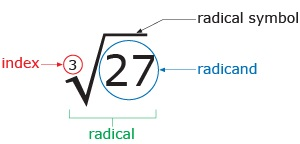
\includegraphics[scale=.7]{radical.jpg}
\end{center}

*Squareroots don't have an index because we assume it's 2\\

The \textbf{radical} tells us that we're looking for identical factors.\\

The \textbf{index} tells us how many identical factors we're looking for.\\

the \textbf{radicand} is a number that needs to be factored so we can pull out the identical ones.\\

\textbf{Example:} $\sqrt[3]{125}=\sqrt{5\cdot5\cdot 5} \Longrightarrow$ since the index is 3, and there are 3- 5's $\Longrightarrow \sqrt[3]{5\cdot5\cdot5}=5$\\

\pagebreak

\section*{Simplifying Radical Expressions}

\begin{center}
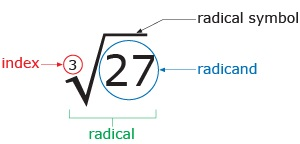
\includegraphics[scale=.7]{radical.jpg}\\
\end{center}

To simplify radical expressions follow these steps\\

\textbf{Step 1:} determine the index\\

\textbf{Step 2:} factor the radicand\\

\textbf{Step 3:} pull out repeated factors of the amount of the index\\

\textbf{Step 4:} all other factors stay inside the radical\\

\textbf{Examples:} Simplify the radical, keep track of the index\\

\begin{multicols}{2}
\textbf{We try:}\\

\begin{enumerate}
	\setlength\itemsep{1cm}

	\item $\sqrt[3]{8}$\\
	
	
	\item $\sqrt[4]{48}$\\
	
	
	\item $\sqrt[3]{27}$\\
	
	
	\item $\sqrt[3]{27x^5}$\\
	
		
\textbf{You Try:}\\
	
	\item  $\sqrt[3]{120}$ \\
	
	
	\item $\sqrt[4]{162y^4}$\\
	
	
	\item $\sqrt[4]{32}$\\
	
	
	\item $\sqrt[3]{162n^7}$\\
	
	

\end{enumerate}
\end{multicols}

 \textbf{Challenge Problem:} $\sqrt[5]{800h^{11}}$

\section*{Add \& Subtract Radical Expressions}

When adding and subtracting radical expressions, treat the radical like a variable whenever possible.\\

$$\sqrt{a} + \sqrt{a} = 2\sqrt{a}$$

The roots need to be exactly the same (i.e. same index, same radicand) to be able to add or subtract.\\

\textbf{Example 1:} $5\sqrt{7} - 3 \sqrt{7} = 2\sqrt{7}$\\

\vspace{1cm}

Sometimes the radical needs to be simplified before adding or subtracting.\\

\textbf{Example 2:} $\sqrt{3} + \sqrt{12}=$\\

\vspace{1cm}

\hrulefill

\textbf{You Try:}\\

\begin{enumerate}

	\item $8\sqrt{h}+ 9\sqrt{h}=$\\
	
	\item $2\sqrt{x} - \sqrt{x}=$\\
	
	\item $6\sqrt{p} - 10 \sqrt{p}=$\\
	
	\item $\sqrt[3]{81} + \sqrt[3]{3}=$\\
	
	\item $\sqrt{8} + \sqrt{32} - \sqrt{2}=$\\
	
\end{enumerate}

\section*{Multiplication \& Division with Radical Expressions}

What happens when we multiply or divide radical expressions?\\

You got an idea of what it's like to multiply roots when you learned to simplify radicals. The concept bridges over.\\

If two roots (with the same index) are multiplied, just multiply the inside numbers. 

$$\sqrt{a} \cdot \sqrt{b} = \sqrt{a \cdot b}$$

\textbf{Example 1:} $\sqrt[5]{8} \cdot \sqrt[5]{4}=$\\

\vspace{1cm}

\textbf{Example 2:} $3\sqrt{5} \cdot 4 \sqrt{6}=$\\

\vspace{1cm}

\textbf{Example 3:} $(2+\sqrt{h})(5+\sqrt{h})=$\\

\vspace{1cm}

\hrulefill

Dividing is just as easy. The square-root symbol can be either broken or put together to the top and bottom.
	
$$\sqrt{\frac{a}{b}}= \frac{\sqrt{a}}{\sqrt{b}}$$

\textbf{Example 3:} $\sqrt{\frac{16}{25}}$

\vspace{1cm}

\textbf{Example 4:} $\sqrt{\frac{8}{100}}$

\vspace{1cm}

\hrulefill
	

\textbf{You Try:}

\begin{enumerate}
\begin{multicols}{2}

	\item $\sqrt{10} \cdot \sqrt{10}=$\\
	
	\item $\sqrt{12} \cdot \sqrt{4}=$\\
	
	\item $(-1 + \sqrt{3})(8 - \sqrt{6})=$\\
	
	\item $\sqrt{\frac{3}{4}}=$\\
	
	\item $\sqrt{\frac{9}{4}}=$\\
	
	\item $\sqrt{\frac{25}{75}}=$\\
\end{multicols}
\end{enumerate} 



\section*{Rational Exponents}

Rational = Fraction \\

What does it mean to have a fraction in the exponent?\\

\begin{center}
\begin{tikzpicture}[scale=3]

	\draw (0,0) -- (2,0) -- (2,2) -- (0,2) -- cycle;
	\node at (1,1){area=s};
	\node at (1,-.5){$\sqrt{s}$};
	\node at (-.5,1){$\sqrt{s}$};
	

\end{tikzpicture}
\end{center}

%\begin{center}
%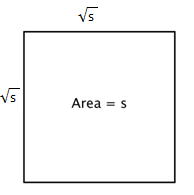
\includegraphics[scale=1]{square.png}
%\end{center}

We know the are of a square is $length \times width$, in this case length and width are the same, so $length^{2}=s$. To find out the length we need to use the inverse operation, the squareroot. So $length=\sqrt{s}$\\

This makes sense because $\sqrt{s} \sqrt{s} = \sqrt{s^2} = s$\\

(or $\sqrt{s} \sqrt{s} = \sqrt{s}^2=s$ they're both the same.)\\

Using our \textbf{properties of exponents} we can see that if we write $$s^{\frac{1}{2}} \cdot s^{\frac{1}{2}}=s$$ since we add the exponents. From here we learn that $\sqrt{s}=s^{\frac{1}{2}}$\\

Having a fraction in the exponent is called a \textbf{RATIONAL EXPONENT.} A \textit{rational exponent} is just another way to write a root. 

\begin{LARGE}
	$$\sqrt{n}= n^{\frac{1}{2}}$$

\end{LARGE}


or more generically, for any index $a$\\

\begin{LARGE}

	$$\sqrt[a]{n^b}=n^{\frac{b}{a}}$$ 
	
\end{LARGE}

OMG that looks scary...

\pagebreak

\textbf{Board Work:} Convert the following from radical form into rational exponent form.\\

$\sqrt[3]{9^2}=9^{\frac{2}{3}}$\\ 

$\sqrt[6]{j^5}=j^{\frac{6}{5}}$\\

$\sqrt[10]{3^3 \cdot k^7}=$\underline{\hspace{2in}}\\


\hrulefill

\textbf{You Try:} Convert the following radical expressions into rational exponent expressions.\\

\begin{enumerate}
\begin{multicols}{2}

\item $\sqrt{7}=$\\

\item $\sqrt{h^3}$\\

\item $\sqrt[3]{27j^3}$\\

\item $\sqrt[5]{k^{10}}$\\


\end{multicols}
\end{enumerate}

\hrulefill

\textbf{You Try:} Convert the rational exponent into a radical -- You don't need to simplify

\begin{enumerate}[resume]
\begin{multicols}{2}

\item $8^{\frac{1}{2}}$\\

\item $3^{\frac{7}{8}}$\\

\item $(5h)^{\frac{3}{2}}$\\

\item $(10k^2)^{\frac{1}{3}}$\\

\end{multicols}
\end{enumerate}

\hrulefill

\textbf{You Try:} Using the properties of exponents you know, simplify the rational exponential expressions

\begin{enumerate}[resume]
\begin{multicols}{2}

\item $6^{3^{\frac{1}{3}}}$\\

\item $16m^{2^{\frac{1}{4}}}$\\

\item $4^{\frac{1}{2}^{\frac{3}{5}}}$\\

\item $(20k^2)^{\frac{7}{10}}(2k)$\\

\end{multicols}
\end{enumerate}



\section*{Put it Together}
Use the properties of exponents to convert, and simplify the radicals and rational exponents. \\

\textbf{The Product Property:} $a^m\cdot a^n=a^{(m+n)}$\\

\hspace{1in} $8^{\frac{1}{2}} \cdot  8^{\frac{3}{2}}=$\\

\vspace{1cm}

\textbf{The Product Property 2:} $(a\cdot b)^m=a^m\cdot b^m$\\

\hspace{1in}$\left(5x\right)^{\frac{3}{2}}=$\\

\vspace{1cm}

\textbf{The Power Property:} $\left(a^m\right)^{n}=a^{(m\cdot n)}$\\

\hspace{1in} $\left(h^{\frac{5}{7}}\right)^{\frac{6}{5}}=$\\

\vspace{1cm}

\textbf{The Quotient Property:} $\frac{a^m}{a^n}=a^{m-n}$\\

\hspace{1in} $\left(\frac{3^{\frac{3}{2}}}{3^{\frac{1}{2}}}\right)=$\\

\vspace{1cm}

\textbf{The Negative Property:} $a^{-b}=\frac{1}{a^{b}}$ \hspace{1cm} or \hspace{1cm} $\frac{1}{a^{-b}}=a^b$\\

\hspace{1in} $(81)^{-\frac{1}{2}}=$\\

\vspace{1cm}

\textbf{Power of a Quotient Property:} $\left(\frac{a}{b}\right)^c=\frac{a^c}{b^c}$\\

\hspace{1in} $\left(\frac{9}{4}\right)^{\frac{1}{2}}=$\\

\vspace{1cm}


\pagebreak

\section*{Evaluating Rational Exponents}

3-Step process for evaluating rational exponential expressions. $a^{\frac{m}{n}}$

\begin{enumerate}

	\item Factor the base of the exponent 
	
	\item Determine the ratio of bases $\frac{m}{n}$
	
	\item Pull out the ratio amount of the bases. 

\end{enumerate}

\textbf{Example:} $\left(216\right)^{\frac{2}{3}}$\\

	\begin{enumerate}
	
		\item $\left(216\right)^{\frac{2}{3}}= \left( 2 \cdot 2 \cdot 2 \cdot 3 \cdot 3 \cdot 3\right)^{\frac{2}{3}}$\\
		
		\item Ratio = $\frac{2}{3}$\\
		
		\item Pull out $\frac{2}{3}$ of each factor  -- $\left( 2 \cdot 2 \cdot 2 \cdot 3 \cdot 3 \cdot 3\right)^{\frac{2}{3}}= 2 \cdot 2 \cdot 3 \cdot 3 = 36$
	
	
	\end{enumerate}

\hrulefill

\textbf{You Try:} Evaluate the rational exponential expressions. Keep an eye out for properties of exponents.\\

\begin{multicols}{2}
\begin{enumerate}
		\setlength\itemsep{1cm}

\item $25^{\frac{1}{2}}$\\

\item $1000^{\frac{2}{3}}$\\

\item $121^{\frac{3}{2}}$\\

\item $49^{-\frac{1}{2}}$\\

\item  $32^{\frac{3}{5}}$\\

\item $16^{-\frac{-5}{2}}$\\

\item $0.04^{\frac{1}{2}}$\\

\item $\left(\frac{1}{125}\right)^{-\frac{1}{3}}$

\end{enumerate}
\end{multicols}

\pagebreak

\section*{Review}

\textbf{Properties of Exponents:} Use the properties of exponents to simplify the exponential expressions. Make sure there are no negative exponents.\\

	\begin{enumerate}
		\begin{multicols}{2}
			
			\item $f^3 \cdot f^6$\\
			
			\item $(5h)^4=$\\
			
			\item $(m^4)^8=$\\
			
			\item $\frac{t^6}{t^4}$\\
			
			\item $\frac{k^2}{k^6}$\\
			
			\item $109745^0=$\\
			
			\item $\left(\frac{2}{9}\right)^{6}=$\\
			
			\item $2^{-4}=$\\
		
		\end{multicols}
	\end{enumerate}

\textbf{Radical Expressions:} Simplify the radical expressions by factoring.\\

	\begin{enumerate}[resume]
		\begin{multicols}{2}
		
			\item $\sqrt{9}$\\
			
			\item $\sqrt{50}$\\
			
			\item $\sqrt[3]{27}$\\
			
			\item $\sqrt[3]{81}$\\
			
			\item $\sqrt{25m^3}$\\
			
			\item $\sqrt[3]{54h^6}$\\
			
		
		\end{multicols}	
	\end{enumerate}
	
\textbf{Operations with Radicals:} Use properties of radicals to simplify the expressions.\\

	\begin{enumerate}[resume]
		\setlength\itemsep{1cm}
		\begin{multicols}{2}
			
			\item $5\sqrt{3}+3\sqrt{3}$\\
			
			\item $9\sqrt[3]{9}-11\sqrt[3]{9}$\\
			
			\item $\sqrt{2} \cdot \sqrt{3}$\\
			
			\item $\sqrt{8m} \cdot \sqrt{2m}$\\
			
			\item $\sqrt[5]{2^{6}j^{8}} \cdot \sqrt[5]{2j^2}$\\
			
			\item $\sqrt{\frac{64}{81}}$\\
		
		\end{multicols}	
	\end{enumerate}	
	
\pagebreak

\textbf{Rational Exponents:} Convert the radical into a rational exponent.\\

	\begin{enumerate}[resume]
		\begin{multicols}{2}
		
			\item $\sqrt{2}$\\
			
			\item $\sqrt{5^2}$\\
			
			\item $\sqrt[3]{k^3}$\\
			
			\item $\sqrt[10]{m^7}$\\
			
			\item $\sqrt[4]{h^3b^5}$\\
			
			\item $\sqrt[3]{p}$\\

		\end{multicols}	
\end{enumerate}	

\textbf{Properties of Exponents on Rational Exponents:} Use the properties of exponents to simplify the rational exponents.\\

	\begin{enumerate}[resume]
		\begin{multicols}{2}
		
		\item $h^{\frac{2}{3}} \cdot h^{\frac{2}{3}}$\\
		
		\item $\left(8g\right)^{\frac{7}{12}}$\\
		
		\item $\left(m^6\right)^{\frac{5}{4}}$\\
		
		\item $\left(\frac{9}{16}\right)^{\frac{1}{2}}$\\

		\end{multicols}	
	\end{enumerate}	

\textbf{Evaluating Rational Exponential Expressions:} Evaluate the rational exponential Expression.\\

	\begin{enumerate}[resume]
		\setlength\itemsep{1cm}
	
		\item $9^{\frac{3}{2}}$\\
		
		\item $27^{\frac{2}{3}}$\\
		
		\item $64^{\frac{2}{3}}$\\
		
		\item $216^{\frac{2}{3}}$\\
		
		\item $32^{\frac{6}{5}}$\\
	
	\end{enumerate}
	
\section*{Test Review}

Mr. Wolf \hfill NAME:\underline{\hspace{3in}}\\ 
Pre-Calculus \\ 
CMSD-JFK \hfill DATE:\underline{\hspace{2in}}\\
2014-2015

\hrulefill

\textbf{Simplify the exponential expression using properties of exponents} (1 point each)\\

\begin{enumerate}
	\begin{multicols}{2}

		\item $j^5 \cdot j^8=$\\
		
		\item $(k^2m)^{8}=$\\
		
		\item $\left(\frac{h}{k}\right)^{6}=$\\
		
		\item $\left(g^5 \right)^{8}=$\\
		
		\item $6^{-4}=$\\
		
		\item $\frac{7}{8}^{-2}=$\\
		
		\item $ 9^0=$\\
		
		\item $0^0=$\\
		
	\end{multicols}
\end{enumerate}

\textbf{Simplify the radicals} (2 points each)\\

\begin{enumerate}[resume]
	\begin{multicols}{2}

		\item $\sqrt{16}$\\
		
		\item $\sqrt{18}$\\
		
		\item $\sqrt[3]{16}$\\
		
		\item $\sqrt[3]{72}$\\
	\end{multicols}
\end{enumerate}

\textbf{Simplify the radical expressions using properties of radicals} (1 point each)\\

\begin{enumerate}[resume]
	\begin{multicols}{2}
	
		\item $\sqrt{2}	\cdot \sqrt{32}$\\
		
		\item $\sqrt[3]{2} \cdot \sqrt[4]{32}$\\
		
		\item $\sqrt{2} + \sqrt{2}$\\
		
		\item $12\sqrt{10} - 17\sqrt{10}$\\
	
	\end{multicols}
\end{enumerate}

\pagebreak

\textbf{Convert from radical to rational exponent} (2 points each)\\

\begin{enumerate}[resume]
	\begin{multicols}{2}
	
		\item $\sqrt{8}$\\
		
		\item $\sqrt[3]{7^2}$\\
		
		\item $\sqrt[5]{k^3}$\\
		
		\item $\sqrt[4]{2^5m^9}$\\

	\end{multicols}
\end{enumerate}


\textbf{Simplify the expressions using properties of exponents and rational exponents} (2 points each)\\

\begin{enumerate}[resume]
	\begin{multicols}{2}

		\item $\left( 5^3 \right) ^{\frac{1}{8}}$\\
		
		\item $\left( 3k \right) ^{\frac{1}{2}}$\\
		
		\item $\left( \frac{9}{2} \right) ^{\frac{3}{2}}$\\
		
		\item $p^{\frac{2}{7}} \cdot p^{\frac{3}{7}}$\\
		
		\item $\left(\frac{3}{2}\right)^{-\frac{5}{4}}$\\
		
		\item $\left(7^{\frac{1}{2}}d\right)^{\frac{1}{3}}$\\

	\end{multicols}
\end{enumerate}

\textbf{Evaluate the exponential expression} (2 points each)

\begin{enumerate}[resume]
	\begin{multicols}{2}
	
		\item $16^{\frac{1}{2}}$\\
		
		\item $25^{\frac{3}{2}}$\\
		
		\item $100^{\frac{5}{2}}$\\
		
		\item $32^{\frac{2}{5}}$\\
		
	\end{multicols}
\end{enumerate}

\hrulefill

\textbf{Pre-assessment:} This place will be extra credit on the real test.\\

The function $f(x)=2^x$ is an exponential function. What happens to the $y$ value as $x$ increases? What happens to the $y$ value as $x$ decreases? \\

\vspace{1in}

Will the graph go below 0? If not how can we change it to go below 0?\\

\section*{Rational Exponents \& Radicals Test}

Mr. Wolf \hfill NAME:\underline{\hspace{3in}}\\ 
Pre-Calculus \\ 
CMSD-JFK \hfill DATE:\underline{\hspace{2in}}\\
2014-2015\\


\textbf{Simplify the exponential expression using properties of exponents} (2 point each)\\

\begin{enumerate}
	\setlength\itemsep{1cm}
	\begin{multicols}{2}

		\item $j^4 \cdot j^7=$\\
		
		\item $(k^3m)^{9}=$\\
		
		\item $\left(\frac{2h}{k}\right)^{5}=$\\
		
		\item $\left(g^4 \right)^{7}=$\\
		
		\item $b^{-5}=$\\
		
		\item $\left(\frac{9}{10}\right)^{-8}=$\\
		
		\item $ 100^0=$\\
		
		\item $(-14)^0=$\\
		
	\end{multicols}
\end{enumerate}

\textbf{Simplify the radicals} (4 points each)\\

\begin{enumerate}[resume]
	\begin{multicols}{2}

		\item $\sqrt{32}$\\
		
		\item $\sqrt{48}$\\
		
		\item $\sqrt[3]{32}$\\
		
		\item $\sqrt[3]{48}$\\
	\end{multicols}
\end{enumerate}

\textbf{Simplify the radical expressions using properties of radicals} (2 point each)\\

\begin{enumerate}[resume]
	\begin{multicols}{2}
	
		\item $\sqrt{3}	\cdot \sqrt{27}$\\
		
		\item $\sqrt[3]{3} \cdot \sqrt[3]{27}$\\
		
		\item $\sqrt{5} + 2\sqrt{5}$\\
		
		\item $\sqrt{8} - 9\sqrt{8}$\\
	
	\end{multicols}
\end{enumerate}

\pagebreak

\textbf{Convert from radical to rational exponent} (4 points each)\\

\begin{enumerate}[resume]
	\begin{multicols}{2}
	
		\item $\sqrt{7}$\\
		
		\item $\sqrt[3]{h^4}$\\
		
		\item $\sqrt[5]{m^12}$\\
		
		\item $\sqrt[4]{2^{10}p}$\\

	\end{multicols}
\end{enumerate}


\textbf{Simplify the expressions using properties of exponents and rational exponents} (4 points each)\\

\begin{enumerate}[resume]
	\begin{multicols}{2}

		\item $\left( p^4 \right) ^{\frac{1}{8}}$\\
		
		\item $\left( 4k \right) ^{\frac{1}{4}}$\\
		
		\item $\left( \frac{5}{4} \right) ^{\frac{5}{4}}$\\
		
		\item $g^{\frac{3}{8}} \cdot p^{\frac{1}{2}}$\\
		
		\item $\left(\frac{2}{3}\right)^{-\frac{9}{4}}$\\
		
		\item $\left(8^{\frac{3}{2}}d\right)^{\frac{2}{3}}$\\

	\end{multicols}
\end{enumerate}

\textbf{Evaluate the exponential expression} (4 points each)

\begin{enumerate}[resume]
	\begin{multicols}{2}
	
		\item $49^{\frac{1}{2}}$\\
		
		\item $25^{\frac{5}{2}}$\\
		
		\item $100^{\frac{3}{2}}$\\
		
		\item $32^{\frac{3}{5}}$\\
		
	\end{multicols}
\end{enumerate}

\hrulefill

\textbf{EXTRA CREDIT:} Simplify the expression (10 points) -- Must be completely correct.\\

$$\left( \frac{2xy^2z^{-5}}{5z^{-2}y^7} \right) \cdot \left( \frac{2z^5y^{-23}}{5x^{-1}y^{-18}z^8} \right)^{-1}$$



\end{document}
